\documentclass[11pt]{article}
\pdfinfoomitdate=1\pdftrailerid{}
\usepackage[letterpaper,margin=.7in,headheight=15pt,headsep=18pt,footskip=24pt]{geometry}
\usepackage[T1]{fontenc}\usepackage{lmodern,amsmath,amssymb,array,booktabs,fancyhdr,tikz,needspace}
\usetikzlibrary{arrows.meta,decorations.markings}
\renewcommand{\familydefault}{\sfdefault}\setlength{\parindent}{0pt}\setlength{\parskip}{5pt}
\pagestyle{fancy}\fancyhf{}\fancyhead[L]{\small Week NN / Who beat whom / Facilitator guide}
\fancyfoot[L]{\scriptsize Bellingham Math Circle / Week NN / FNN-FAC-v1}\fancyfoot[R]{\thepage}
\renewcommand{\headrulewidth}{0.4pt}
\newcommand{\head}[1]{\par\needspace{6\baselineskip}\vspace{2pt}\textbf{\large #1}\par}
\newcommand{\sub}[1]{\par\needspace{3\baselineskip}\textbf{#1}\par}
\newcommand{\bt}{\,$\to$\,\allowbreak}
\tikzset{mid/.style={postaction={decorate},decoration={markings,mark=at position .58 with {\arrow{Stealth[length=5pt,width=5pt]}}}},
  pl/.style={circle,draw,line width=.7pt,minimum size=7.5mm,inner sep=0pt,font=\footnotesize\bfseries}}
\emergencystretch=1.5em\hyphenation{rabbit}
\begin{document}
\head{Mathematical overview: every tournament has a line-up}
\textbf{The model.} Every two players play exactly one game, one of them wins, and no result is revised. An arrow points from the winner to the loser; a player's wins are the arrows leaving it. A \emph{line-up} is a row of all the players in which each player beat the next one (players further apart are not compared). A \emph{king} can get to every other player by one arrow or two arrows in a row.

\textbf{1. A line-up always exists (R\'edei 1934).} Proof by insertion. Suppose some players stand in a line-up $P_1,\dots,P_k$ and a new player $X$ has played each of them. If $X$ beat $P_1$, $X$ goes in front; if $X$ lost to $P_k$, at the back. Otherwise $X$ lost to $P_1$ and beat $P_k$; if $P_j$ is the first player $X$ beat, then $j\ge2$ and $P_{j-1}\to X\to P_j$, so $X$ fits between them. Add the players one at a time. The argument uses every game; if two players never met, a line-up can fail. The frog, the pig and player $X$ on the pages perform exactly this step.

\textbf{The line-up is unique exactly when the results are a strict ranking.} In a ranking the unbeaten player must stand first, the next one second, and so on. If no three players beat each other in a circle, ``$a$ beat $b$, $b$ beat $c$'' forces ``$a$ beat $c$'', so the results are a ranking. Thus a non-ranking contains a circle of three, which alone has three line-ups; with more players, set aside one player outside the circle, find two line-ups of the rest by induction, and insert the set-aside player into each.

\textbf{R\'edei also proved that the number of line-ups is always odd.} Proof idea (Schweser, Stiebitz and Toft, Section~1): reversing one arrow changes the number by an even amount, a ranking has exactly one, and reversing arrows one at a time reaches every tournament. The even-change step is a real theorem that no child is expected to prove; we checked oddness for all tournaments of up to six players. Four players have 1, 3 or 5 line-ups (24, 16 and 24 of the 64 ways to lay arrows on the K--1 board), and each four-player tournament has one of four shapes, fixed by its win list: $0,1,2,3$ (a ranking, 1 line-up), $1,1,1,3$ and $0,2,2,2$ (3 each), $1,1,2,2$ (5). It has 5 exactly when its arrows go round all four players in one circle. A player can start a line-up exactly when it can get to every other player along arrows, in any number of steps. The players who can do so beat everyone else, and when there are several of them their arrows go round one circle through all of them (Camion 1959): start anywhere on that circle, go round it, then continue with a line-up of the rest.

\textbf{2. A player with the most wins is always a king (Landau 1953).} If $x$ has the most wins and cannot get to $y$ in one or two arrows, then $y$ beat $x$ and every player $x$ beat (otherwise $x\to z\to y$), so $y$ has more wins than $x$: impossible. Hence every tournament has a king. The converse fails: in grades 4--5 Problem 5 a one-win player is a king and a three-win player is not.

\textbf{No tournament has exactly two kings.} An unbeaten player is the only king, since nobody can get to it. Otherwise take a king $x$. Among the players who beat $x$, a top scorer in their games with each other is a king of that group (theorem 2), and so a king of everyone: it beat $x$ and gets to $x$'s victims through $x$. Call it $y$; repeating from $y$ gives a third king, who beat $y$ and so is not $x$. By enumeration, four players have 1 or 3 kings, five have 1, 3, 4 or 5, six have 1, 3, 4, 5 or 6; Maurer (1980) treats every number of players.

\textbf{3. Which win lists can happen (Landau 1953).} A list sorted from smallest is the win list of some tournament exactly when, for every $k$, its $k$ smallest numbers add to at least $k(k-1)/2$ (0, 1, 3, 6, 10, 15, \dots), with equality for the whole list. \emph{A failing list cannot happen:} the $k$ weakest players play $k(k-1)/2$ games among themselves, each giving one of them a win. (Equivalently, the $k$ strongest win at most their games among themselves plus all their games against the rest.) \emph{A passing list always happens} (proof idea): give the numbers to the players and start from any tournament, say a ranking. From the players with too many wins, follow arrows forward. If you reach a player with too few, reverse every arrow on that path: only its two ends change, by one win each, so the wins come closer to the list. If you cannot reach one, the players you can reach lost every game against the others, so they won exactly the games among themselves, while the list gives them fewer; then the list fails the test. Our script runs this with every choice random for every list of up to eight players. Four players have 4 possible sorted lists, five have 9, six have 22. Every printed list has the right total, so the total alone never decides one.

\textbf{What children discover.} Experiments (playing, lining up, listing line-ups, finding kings, building tournaments for win counts) lead to conjectures (a line-up always exists; a top scorer is a king; never two kings; four players give 1, 3 or 5 line-ups; a test for win lists) and to explanations children can give with cards or drawings: the joining argument, two unbeaten players played each other, 6 wins cannot be shared equally by 4 animals, the top-scorer argument, a group with fewer wins than its own games. The odd count in general, the passing half of Landau's test and the full list of king counts stay adult knowledge.

\textbf{Band map.} \emph{K--1} (no reading; counting to 6): play four animals on the big board and line them up, fit in the frog and the pig, count line-ups of three animals (1 or 3), build boards with one line-up and with the most (5), find who can be first, meet three impossibilities (equal wins for four, two unbeaten animals, no line-up). \emph{Grades 2--3} (short sentences, some adult reading): record by drawing, find the tournaments with one line-up, show a newcomer can never be shut out, then kings, their possible numbers for four players, and why a top scorer is one. \emph{Grades 4--5} (independent reading, small sums): the general joining proof, every line-up of the four shapes, kings and why never two, which win lists happen and Landau's test, and why four players never have 2 or 4 line-ups.

Every answer below was recomputed from the final pages' figure files by \texttt{check\_guide.py}.

\head{Preparation, shared launch and pacing}
\textbf{Status.} Draft for organizer review; unpiloted. Untried physically: the 75\,mm arrow cards in the big board's lanes and on the mats, the K--1 Problem~2 flow from the frog mat to the pig mat to the strip, the pace of rock-paper-scissors, and all time estimates.

\textbf{Print.} US Letter, single-sided, at actual size (100\%). \emph{Packets}: K--1 (5 pages) one per pair; grades 2--3 (6 pages) and 4--5 (8 pages) one per child, worked in pencil. K--1 page~1 is the big board, the pair's mat for Problems 1, 5, 6, 8, 9 and 10: four 4\,cm animal squares joined by dashed lanes 2.3\,cm wide, 10.8\,cm long on the sides and 15.3\,cm on the diagonals. \emph{Materials file} \texttt{materials.pdf}: five landscape pages, page~1 in color if possible, card stock if the printer takes it. Check the 100\,mm scale bar on page~1 after printing.\par
{\renewcommand{\arraystretch}{1.12}\small\begin{tabular}{@{}c>{\raggedright\arraybackslash}p{3.3cm}>{\raggedright\arraybackslash}p{5.0cm}>{\raggedright\arraybackslash}p{7.4cm}@{}}
\toprule
Page & Object & Size & Print and use\\\midrule
1 & Animal cards & three sets of cat, dog, bear, rabbit, frog, pig; 40\,mm squares, like the big board's animal squares & one sheet per table of up to three pairs (one set per pair), every band\\
2 & Arrow cards & 18 cards, 75\,$\times$\,20\,mm & one sheet per K--1 pair: 15 in use (6 on the big board, 4 for the frog, 5 for the pig), 3 spare\\
3 & Line-up strip (K--1) & six 44\,mm boxes in two parts, butted or taped end to end & one per K--1 pair (Problems 1, 2, 4, 6)\\
4, 5 & K--1 Problem 2: frog; K--1 Problem 2: pig & full-size mats of the Problem~2 picture; not cut & one of each per K--1 pair\\\bottomrule
\end{tabular}}\par
A K--1 pair gets materials pages 2--5 and one set from page~1; an older table gets only page~1. The arrow cards fit the big board's lanes with room to spare; the two diagonal cards overlap a little at the center, which is fine. Older children draw arrows on their pages. Arrow cards are optional there, for laying out a first tournament: grades 2--3 use 6 per pair (one sheet serves three pairs), grades 4--5 use 10 per pair if they lay out the five-animal tournament first, otherwise none. Older children write initials in the line-up boxes; C, D, B, R, F, P all differ. Also needed: pencils and erasers, and a whiteboard for the launch.

\textbf{Preparation time.} Cutting is the only work: about 5 minutes per sheet of 18 cards with scissors (neighboring cards share cut lines) and 2 per line-up strip; the mats are not cut. For three K--1 pairs and two older tables of three pairs (3 animal sheets, 3 arrow sheets, 3 strips) that is about 40 minutes plus printing, less with a paper cutter. The kit is reusable. Untested estimates.

\textbf{Staffing.} At least two adults: one at the K--1 table for two or three pairs, and one moving between the older tables, mostly at grades 2--3. The K--1 adult reads each problem aloud, referees rock-paper-scissors (ties are replayed; once an arrow card is down it stays), and writes initials or marks in recording boxes when asked. The children choose every arrow, order and place. When a child proposes a line-up, the adult points to one pair of neighbors and asks who won that game, rather than saying yes or no. Grades 2--3 need an adult nearby to read Problems 3 and 7 and check claimed line-ups. Grades 4--5 work largely alone; an adult listens to the explanations in Problems 3--4, 6, 8, 12 and 13. Adult reading and recording are ordinary support; an adult choosing the next animal is a signal to use fewer animals, or cards instead of drawings.

\textbf{Shared launch (5 minutes).} Let children handle the animal and arrow cards for a minute. Then three volunteer children are the players, so the example is no task's instance. Two of them play rock-paper-scissors (replay a tie), and a child lays an arrow card on the floor between them, from the winner to the loser: ``This says Kai beat Lu. It stays, even if Lu wants a rematch.'' The cards are small, so an adult draws each result on the whiteboard as dots and arrows, as the older tables record; the whiteboard is what everyone watches. Play the other two games. Ask the three to stand in a row in which each person beat the next, and check each neighbor pair by its arrow; show one row that fails. Stop after one good row: do not ask whether there is another, or whether a row can always be made. At the K--1 table a child then lays one arrow card in a lane of the big board.
\begin{center}
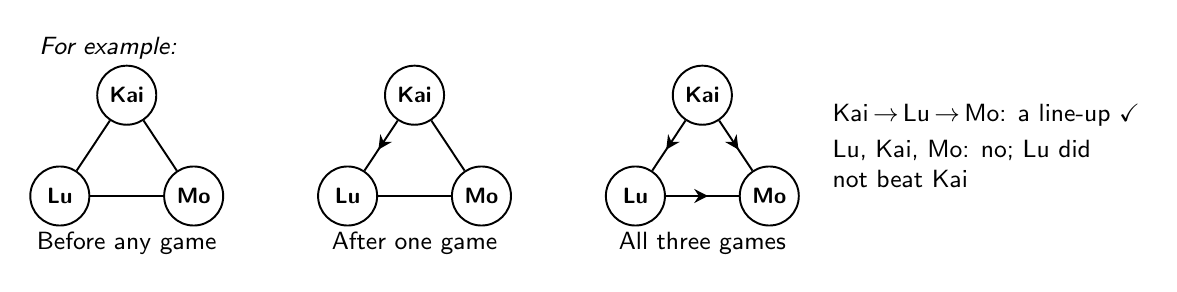
\begin{tikzpicture}[x=.85cm,y=.8cm]
\node[font=\small\itshape,anchor=west] at (-0.45,2.35) {For example:};
\foreach \i/\ox/\cap in {1/0/Before any game, 2/4.3/After one game, 3/8.6/All three games} {
  \node[pl] (K\i) at (\ox+1,1.6) {Kai};
  \node[pl] (L\i) at (\ox,0) {Lu};
  \node[pl] (M\i) at (\ox+2,0) {Mo};
  \node[font=\small] at (\ox+1,-0.75) {\cap};
}
\draw[line width=.7pt] (K1)--(L1); \draw[line width=.7pt] (L1)--(M1); \draw[line width=.7pt] (K1)--(M1);
\draw[line width=.7pt,mid] (K2)--(L2); \draw[line width=.7pt] (L2)--(M2); \draw[line width=.7pt] (K2)--(M2);
\draw[line width=.7pt,mid] (K3)--(L3); \draw[line width=.7pt,mid] (L3)--(M3); \draw[line width=.7pt,mid] (K3)--(M3);
\node[font=\small,align=left,anchor=west] at (11.4,0.8) {Kai\bt Lu\bt Mo: a line-up \checkmark\\[2pt] Lu, Kai, Mo: no; Lu did\\not beat Kai};
\end{tikzpicture}
\end{center}

\textbf{Return-visit launch (2 minutes).} Kings and win counts each bring a new procedure. Before kings (2--3 Problem~7, 4--5 Problem~5), three children stand as P, Q and R with arrow cards laid as in the pages' small P\,$\to$\,Q\,$\to$\,R\,$\to$\,P picture, and walk from one child to another along one arrow, or two arrows in a row, never against an arrow: ``Can Q get to P?'' (Q\,$\to$\,R\,$\to$\,P.) Here everyone is a king and everyone won one game, so the demonstration says nothing about top scorers or any page's answer. Before win counts (4--5 Problem~9), the same three each count the arrows leaving them, and an adult writes 1 in each dot on the whiteboard.

\textbf{A first visit.} After the launch, about 45 minutes at tables and 5 to compare one line-up, one surprise and one question. \emph{K--1}: Problems 1--4 (the six games of Problem 1 take about 10--15 minutes; Problem 2's nine games about 10). Close with Problem 9 as a table question. Return visit: Problems 5--8 and 10. \emph{Grades 2--3}: Problems 1--5, with one or two tournaments in Problem 1 rather than three; Problem 6 as the closing question. Return visit: kings, Problems 7--9. \emph{Grades 4--5}: Problems 1--4, then 5--6 if there is time. Later visits: kings (Problems 5--8, from wherever the first visit stopped), then win counts (Problems 9--12); Problem 13 fits whenever Problem 2 is fresh. A 2--3 child who finishes the kings can join the 4--5 win-count problems; a K--1 child who lines up quickly can try 2--3 Problems 3--5 with cards. Finishing every page is not the goal.

\head{Grades K--1: solutions and hints}
Pictures are described by position on the page. In every answer an arrow means ``beat''.

\sub{Problem 1, page 1: play and line up}
Arrow cards (materials page~2) go in the board's lanes; the line-up is built with animal cards (page~1) on the line-up strip (page~3). Any results are possible, and every board has a line-up (theorem 1). Children may start with the animal that won the most and follow arrows. If a row breaks, ask: ``Who won the game between these two? Find their arrow card.'' If a child is stuck again and again, ask whether they can line up three of the animals first and then fit in the fourth, as the frog does next.

\sub{Problem 2, page 2: the frog and the pig join}
The printed picture is a small layout; play on the full-size frog mat (materials page~4). The four animal cards of the Problem~1 line-up go in its boxes, the frog card on the printed frog, and one arrow card in a lane after each game. The frog always fits (theorem 1). A child's reason: ``The frog lost to the cat and beat the dog, so it goes between them.'' Let the pair point to the frog's place and say why before moving anything, because the frog's arrow cards mean nothing once the animals leave their boxes. Then the five cards, frog included, go in the boxes of the pig mat (page~5), the pig card goes on the printed pig and plays all five the same way, and all six go on the line-up strip. Hints: ``Did the frog beat the first animal? Did it lose to the last one?''; ``Is there an animal the frog lost to, right before one it beat?'' Extension: can the frog fit in more than one place?

\sub{Problem 3, page 2: how many ways for three animals}
Left: 1 way, frog\bt pig\bt rabbit. The frog won both games, so it must be first; the rabbit lost both, so it must be last. Right: 3 ways, cat\bt bear\bt dog, bear\bt dog\bt cat, dog\bt cat\bt bear. Each animal won once, and the arrows go round in a circle, so any animal can start. Hint: ``Can the rabbit be first?'' Extension: can three animals line up in exactly two ways? (No: always 1 or 3.)

\sub{Problem 4, page 3: line up four}
Any one line-up answers each picture; all are listed for checking. There are no recording boxes: children build each line-up with animal cards on the strip (materials pages 1 and 3) and check it with the adult. Hint: ``Which animal could stand first? Whom did it beat?'' Extension: find a second line-up for the same picture.\par
{\renewcommand{\arraystretch}{1.15}\begin{tabular}{@{}l>{\raggedright\arraybackslash}p{14.6cm}@{}}
Top left & only pig\bt cat\bt dog\bt frog (a ranking)\\
Top right & the rabbit beat everyone, so it is first: rabbit\bt frog\bt cat\bt bear; rabbit\bt cat\bt bear\bt frog; rabbit\bt bear\bt frog\bt cat\\
Bottom left & the dog lost every game, so it is last: pig\bt cat\bt rabbit\bt dog; rabbit\bt pig\bt cat\bt dog; cat\bt rabbit\bt pig\bt dog\\
Bottom right & 5 line-ups: dog\bt rabbit\bt bear\bt frog; dog\bt frog\bt rabbit\bt bear; rabbit\bt bear\bt dog\bt frog; bear\bt dog\bt frog\bt rabbit; frog\bt rabbit\bt bear\bt dog
\end{tabular}}

\sub{Problem 5, page 3: only one way}
The results must be a ranking: one animal beat all three others, one of the rest beat the remaining two, and the third beat the last. Example: the cat beat everyone, the dog beat the bear and the rabbit, the bear beat the rabbit; the only line-up is cat\bt dog\bt bear\bt rabbit. 24 of the 64 boards work. Children may describe it as ``best to worst''. Hint: ``What if one animal beat all the others?''

\sub{Problem 6, page 4: as many ways as possible}
Five is the most; every four-animal board has 1, 3 or 5 line-ups. A board has 5 exactly when its arrows go round all four animals in one circle. Example: cat\bt dog\bt bear\bt rabbit\bt cat around the outside, with cat\bt bear and dog\bt rabbit on the diagonals, gives cat\bt dog\bt bear\bt rabbit, dog\bt bear\bt rabbit\bt cat, bear\bt rabbit\bt cat\bt dog, rabbit\bt cat\bt dog\bt bear and dog\bt rabbit\bt cat\bt bear. The diagonals may point either way. K--1 children cannot prove that 5 is the most; their evidence is that no board they try beats it. Children can test line-ups with the cards on the strip; six recording rows leave one spare. Hints: ``Can every animal be first on your board?''; later, if needed, ``Can the arrows go all the way round?''

\sub{Problem 7, page 4: who can be first}
Left: only the dog. It beat all three others, so nobody can stand in front of it. Middle: pig, cat and rabbit, not the bear. The bear lost every game, so nobody can come after it. Right: all four. The arrows frog\bt pig\bt dog\bt bear\bt frog go round every animal, so a line-up can start anywhere on that circle. Adult note: an animal can be first exactly when you can get from it to every other animal along arrows (overview). Hint: ``If the bear is first, who comes next?''

\sub{Problem 8, page 5: winning equally}
Three animals: yes. Each beats one other in a circle, cat\bt dog\bt bear\bt cat or the reverse; these are the only two ways. Four animals: no. There are 6 games, so 6 wins to share, and four equal shares would be one and a half each. Concrete proof: each arrow card is one win for the animal at its tail; hand each card to its winner, and the piles cannot come out equal. Hint: ``How many arrow cards are on the board? Can four animals share them fairly?''

\sub{Problem 9, page 5: two unbeaten animals}
No. Those two animals played each other, and one of them lost that game. Hint: ``Who won the game between those two?''

\sub{Problem 10, page 5: a board with no line-up}
No board works (theorem 1). A child who cannot find a line-up may believe they have succeeded. Check together by building a line-up one animal at a time, as the frog joined: two animals, then a third, then the fourth. ``How do you know for sure?'' fits here: after several boards, ask whether the frog's way of joining could ever fail.

\head{Grades 2--3: solutions and hints}
\sub{Problem 1, page 1: three tournaments}
Results vary; each tournament has a line-up. For each game the two children hold the two animal cards (materials page~1) and play for them; ask children to draw each arrow as soon as its game is played. One or two tournaments are enough for a first visit; the last one played is reused in Problem 3.

\sub{Problem 2, page 2: which have only one line-up}
Top left, 5 line-ups: A\bt C\bt B\bt D, B\bt D\bt A\bt C, C\bt B\bt D\bt A, C\bt D\bt A\bt B, D\bt A\bt C\bt B. Top right, only D\bt B\bt A\bt C (wins 3, 2, 1, 0). Bottom left, only C\bt E\bt A\bt D\bt B (wins 4, 3, 2, 1, 0). Bottom right, 3: B\bt E\bt A\bt C\bt D, B\bt E\bt C\bt D\bt A, B\bt E\bt D\bt A\bt C. So the top right and bottom left have only one: each player beat everyone below it in the win order, so the order is forced. In the other two the second row holds a second line-up. Alphabetical order is never a line-up. Hint: ``Who has to go first? Is there a choice after that?'' Extension: what do the one-line-up tournaments have in common?

\sub{Problem 3, page 3: the frog and the pig join}
Always possible (theorem 1). The frog's and the pig's games are played with their cards from materials page~1. Hints: ``Did the frog beat the first animal? Did it lose to the last?''; ``Is there an animal the frog lost to, just before one it beat?''

\sub{Problem 4, page 3: every place for X}
Top left (X lost to A, B, C and beat D, E): between C and D only. Top right (X lost to all five): after E only. Bottom left (X beat only B): between A and B, and after E. Bottom right (X beat A and D): before A, between C and D, and after E. That is 1, 1, 2 and 3 places. Hint: ``What does X need from the player before it and the player after it?''

\sub{Problem 5, page 4: shut X out}
Impossible. If X beat A, X goes first; if X lost to E, X goes last. Otherwise X lost to A and beat E, so somewhere along the row X goes from losing to winning, and it fits between those two players. The two blank pictures are for attempts. Hints: ``What must happen at the front and at the back for X to be shut out?''; ``If X lost to A and beat E, what happens somewhere in between?''

\sub{Problem 6, page 4: six players with no line-up}
Impossible (theorem 1). Line up any two players, then fit in the others one at a time as in Problems 3--5. A drawn attempt with its line-up found is good evidence; the joining argument is the explanation. Hint: ``How did the frog and the pig always find a place?''

\sub{Problem 7, page 5: find all the kings}
Top left: A, C, D. B won no games, so it gets to nobody. Top right: only C. C beat everyone, so nobody gets to C. Bottom left: A, C, D, E. B beat only A, and A beat C and E, so B never gets to D. Bottom right: all five. Every player won 2 games, and following the star A\bt C\bt E\bt B\bt D\bt A, each beat the next two (not around the drawn pentagon). Hint: ``From B, where can you get by one arrow? By two?'' Arrows are followed forward only.

\sub{Problem 8, page 6: 1, 2, 3 or 4 kings}
1 and 3 kings can be made; 2 and 4 cannot. Problem 7's top right has 1 king and its top left has 3. Not 2: an unbeaten player is the only king, and otherwise there are at least three (overview). Not 4: every four-player tournament has one of four shapes, with 1, 1, 3 and 3 kings. For grades 2--3 the evidence is many failed attempts; the eight squares leave room for them. Hint: ``What happens to the kings when one player beat everyone?''

\sub{Problem 9, page 6: is a top scorer always a king?}
Yes. A child's version: ``Say Sam won the most but can't get to Tia. Then Tia beat Sam. Tia also beat everyone Sam beat, or Sam would get to Tia in two arrows. So Tia won more than Sam, but Sam won the most.'' In Problem 7 every top scorer is a king. Kings need not be top scorers: in the bottom left, A, C and E won 2 games each and are kings, while D won 3.
\head{Grades 4--5: solutions and hints}
\sub{Problem 1, page 1: play five, then the pig}
Results vary; a line-up always exists, and the pig fits in as in Problem 3. For each game the two children hold the two animal cards (materials page~1) and play for them.

\sub{Problem 2, page 1: every line-up}
First square, 5: A\bt C\bt B\bt D, A\bt D\bt C\bt B, B\bt A\bt D\bt C, C\bt B\bt A\bt D, D\bt C\bt B\bt A. Second, 3: B\bt D\bt C\bt A, C\bt B\bt D\bt A, D\bt C\bt B\bt A (A won nothing, so it is last). Third, 1: C\bt A\bt D\bt B (a ranking). Fourth, 3: D\bt A\bt C\bt B, D\bt B\bt A\bt C, D\bt C\bt B\bt A (D beat everyone, so it is first). To know a list is complete, try each player first and follow every possible arrow; a branch ends when the last player beat nobody unused. These four are the four shapes of a four-player tournament, used again in Problems 7 and 13. Hint: ``Have you tried every player first?''

\sub{Problem 3, page 2: places for X, and always?}
Top left (X beat C and E only): between B and C, and between D and E. Top right (X beat only E): between D and E only. Bottom (X beat A and B, lost to C, D, E): in front and at the back only. X can always join (theorem 1). Listen for the three cases: X beat A; X lost to E; or X lost to A and beat E, so somewhere along the row it switches from losing to winning. Hint: ``Where can X go if it beat A? If it lost to E? And if neither?''

\sub{Problem 4, page 2: every tournament?}
Yes, however many players (theorem 1): one player is a line-up, and each new player fits in by Problem 3. ``How do you know for sure?'': does the Problem 3 explanation cover every possible pattern of results? Extension: the number of line-ups is always odd (R\'edei), which Problem 13 tests for four players.

\sub{Problem 5, page 3: find all the kings}
Top left pentagon: A, C, D. Top right pentagon: B, C, D, E. A beat only E, and E beat B and D, so A never gets to C. Bottom left hexagon: all six. Bottom right hexagon: A, D, F. F won only one game, but it beat D, and D beat everyone except F. B won three games yet is not a king: only D beat A, and B lost to D.

\sub{Problem 6, page 3: is a top scorer always a king?}
Yes; the argument is theorem 2 in the overview, and the 2--3 Problem 9 wording works here too. The bottom right hexagon of Problem 5 shows that the converse fails.

\sub{Problem 7, page 4: numbers of kings for four and five players}
Four players: 1 or 3. Examples: Problem 2's third square (C alone) and its first square (A, B, C). Not 4: Problem 2's four shapes have 3, 3, 1 and 1 kings, and every four-player tournament has one of those shapes. Five players: 1, 3, 4 or 5. Examples: one player beat all four (1); Problem 5's top left pentagon (3); its top right pentagon (4; the only win list with four kings is $1,2,2,2,3$); everyone beats the next two going round (5). The spare diagrams are for failed attempts at 2.

\sub{Problem 8, page 4: exactly two kings?}
Never; the argument is in the overview. It uses Problem 6 on a smaller group: if nobody beat everyone, take a king K, find the top scorer among the players who beat K (counting only their games against each other), and check that it is a king of everyone; then repeat from that player to get a third. This is a readiness-dependent extension. Expect many children to offer the unbeaten case (``then only that player is a king'') and evidence from Problem 7; that is a good stopping point. Hint, for a child who wants the rest: ``Suppose nobody beat everyone. Who beat your king, and is one of them a king too?''

\sub{Problem 9, page 5: win counts for five players}
Lists are read from the top dot clockwise. (1) $1,3,1,4,1$: possible. The 4 beat everyone, the 3 beat the three 1s, and the three 1s beat each other in a circle. (2) $0,3,4,0,3$: impossible; the two 0s played each other. (3) $2,2,2,2,2$: possible; each beats the next two clockwise. (4) $4,1,0,4,1$: impossible; the two 4s played each other, so one of them lost a game. Seen from below, the 0 and the two 1s played 3 games among themselves but have only 2 wins. (5) $3,0,3,1,3$: possible. Everyone beat the 0, the three 3s beat the 1, and the 3s beat each other in a circle. Every total is 10, so adding up never decides a case. Hint: ``Which two players are in trouble when they play each other?''

\sub{Problem 10, page 6: win counts for six players}
Lists are read from the top dot clockwise. (1) $4,1,4,1,4,1$: possible. Each 4 beat all three 1s, the 4s beat each other in a circle, and so do the 1s. (2) $0,4,1,5,1,4$: impossible. The 0 and the two 1s played 3 games among themselves but have only 2 wins; from above, the 5 and two 4s won 13 games, but they can win at most 3 among themselves plus 9 against the others. This is a three-player obstruction: there is only one 0 and one 5. (3) $2,3,2,3,2,3$: possible. Each beats the next two clockwise, and in each of the three games straight across the hexagon the 3 beats the 2. (4) $5,0,2,4,2,2$: possible. The 5 beat everyone, everyone beat the 0, the 4 beat the three 2s, and the 2s beat each other in a circle.

\sub{Problem 11, page 7: every list for four and five players}
Four players: $0,1,2,3$; $0,2,2,2$; $1,1,1,3$; $1,1,2,2$. Five players: $0,1,2,3,4$; $0,1,3,3,3$; $0,2,2,2,4$; $0,2,2,3,3$; $1,1,1,3,4$; $1,1,2,2,4$; $1,1,2,3,3$; $1,2,2,2,3$; $2,2,2,2,2$. To know the lists are complete, list every sorted list of numbers from 0 to $n-1$ with the right total (6 or 10). For four players that adds only $0,0,3,3$; for five, $0,0,2,4,4$, $0,0,3,3,4$ and $0,1,1,4,4$. Each of these has two 0s or two top scores. Every survivor needs a built tournament as proof; the 5 squares and 12 pentagons include spares, and children can share the work and pool their tournaments. Hint: ``Can two players both have 0? Both have 4?'' Extension: six players have 22 lists.

\sub{Problem 12, page 8: a test for win lists}
Sort the list from smallest. For each $k$, the $k$ smallest numbers must add to at least 0, 1, 3, 6, 10, 15, \dots, the number of games among $k$ players, and the whole list must add to exactly that number for all the players. A failing list cannot happen, because those $k$ players play that many games among themselves, and each game gives one of them a win. A child may say instead: ``no group can have fewer wins than the games inside the group'', or the top-group version. A likely first proposal is ``at most one 0 and at most one player who beat everyone''. That is enough for four and five players (Problem 11) but not for six: Problem 10's second list passes it and still fails. That every passing list happens is Landau's theorem; the page does not ask for it. Adults can show the path idea from the overview to a child who wants more. Hint: ``Look at the lists you could not build in Problems 9--11. Which group of players is in trouble together?''

\sub{Problem 13, page 8: two or four line-ups?}
Neither. Every four-player tournament has one of the four shapes in Problem 2, with 5, 3, 1 and 3 line-ups. Each win list from Problem 11 allows only one shape. For example, with $1,1,1,3$ the 3 beat everyone, and the other three each won one game among themselves, so they go round in a circle. R\'edei's theorem says the count is always odd. Hint: ``Which tournament in Problem 2 has the same win counts as yours?''

\head{Sources and connections}
L.~R\'edei, ``Ein kombinatorischer Satz'', \emph{Acta Litterarum ac Scientiarum Szeged} 7 (1934), 39--43: a line-up always exists and their number is odd. Not consulted; cited from the outline and from the next source.\par
T.~Schweser, M.~Stiebitz and B.~Toft, ``The Tournament Theorem of R\'edei revisited'', arXiv:2510.10659, consulted October 25, 2026: abstract and Section~1 (R\'edei's odd count, his stronger Theorem 1.1, and the derivation by reversing arrows starting from a ranking).\par
H.~G.~Landau, ``On dominance relations and the structure of animal societies III'', \emph{Bulletin of Mathematical Biophysics} 15 (1953): a top scorer is a king, and the test for win lists. Not consulted.\par
P.~Camion, ``Chemins et circuits hamiltoniens des graphes complets'', \emph{Comptes Rendus de l'Acad\'emie des Sciences Paris} 249 (1959), 2151--2152: the players who can reach everyone go round one circle. Not consulted.\par
S.~B.~Maurer, ``The king chicken theorems'', \emph{Mathematics Magazine} 53 (1980), 67--80: which numbers of kings occur. Not consulted.\par
J.~W.~Moon, \emph{Topics on Tournaments} (1968): line-ups and win lists; sections not checked, not consulted.\par
The insertion, top-scorer and failing-list arguments are the standard ones. The uniqueness induction, the never-two-kings argument and the path sketch of Landau's passing half are written for this guide; the computer checks cover small cases only.\par
Library links: Week 87's three voters make a three-way majority cycle (a three-player circle), Week 24's decks beat each other in a circle, Week 23 sorts by comparisons, and Week 10's return visit walks one-way streets. New here: R\'edei's line-up theorem with its joining proof, kings, and the test for win lists.

\textbf{What to record.} Which problems each table reached, whether K--1 children kept the arrow cards fixed and could check a row by its cards, whether the 75\,mm cards were easy to handle, whether the K--1 Problem~2 flow across the frog mat, pig mat and strip needed adult rescue, how long the games took, and one explanation in a child's words. Keep observations separate from guesses about why.
\end{document}
